\documentclass[a4paper, 12pt]{article}

% -- Language --
\usepackage[spanish]{babel}
\usepackage[utf8]{inputenc}

% ----- Fonts -----
% -- Color --
\usepackage{xcolor}
%\definecolor{azul}{RGB}{00,33,99}
\definecolor{azul}{RGB}{35,72,180}

% -- Page Margin --
\usepackage[margin=1in]{geometry}

% -- Espaciados --
\newcommand{\Pspace}{0.5cm}
\newcommand{\Aspace}{0.2cm}

% -- Imagenes --
\usepackage{graphicx}
\usepackage{float}

% -- Matemáticas --
\usepackage{amsmath, amssymb}

% -- Gráficas --
\usepackage{pgfplots}
\pgfplotsset{compat=1.18}

% -- Código --
\usepackage{listings}
\lstset{
    language=C++,                   % Lenguaje del código
    basicstyle=\ttfamily\small,     % Fuente del código
    keywordstyle=\color{blue},      % Color de palabras clave
    commentstyle=\color{gray},      % Color de comentarios
    stringstyle=\color{red},        % Color de cadenas
    numbers=left,                   % Números de línea a la izquierda
    numberstyle=\tiny\color{gray},
    breaklines=true,                % Permitir saltos de línea
    frame=single                    % Marco alrededor del código
}


\title
{
    Probabilidad 2025-1 \\
    Tareas Parcial 3
    }

    \begin{document}

    \maketitle

    \begin{center}
        \begin{tabular}{r|l}
            \textbf{Expediente} & \textbf{Nombre} \\ \hline
            219208106 & Bórquez Guerrero Angel Fernando \\
            223203899 & Tostado Cortes Dante Alejandro \\
        \end{tabular}
    \end{center}

    \rule{\linewidth}{0.3mm}



    % ---------- Tarea 9 ----------
    \vspace{0.3cm}

    \begin{center}
        { \LARGE Tarea 9}
    \end{center}

    \begin{enumerate}
        % - Problema 1
        \item Comprobar si la siguiente función es de probabilidad \par
        \[
            f(x) =
            \begin{cases}
                \frac{1 / 2}{\sqrt{x}} & 0 < x < 1 \\
                0 & \text{Otro caso}
            \end{cases}
        \]
            % Respuesta:
            \vspace{\Aspace}
            { \color{azul} 
                \[  \int_{0}^{1}\frac{\frac{1}{2}}{\sqrt{x}}dx 
                    = \frac{1}{2} \int_{0}^{1}x^{-\frac{1}{2}}dx
                    = \frac{1}{2} \left[ \frac{\sqrt{x}}{\frac{1}{2}} \Big|_{0}^{1} \right]
                    = \sqrt{x} \Big|_{0}^{1}
                    = \sqrt{1} - \sqrt{0} = 1
                \]
            }
        
        \newpage
        % - Problema 2
        \vspace{\Pspace}
        \item Encontrar la función de distribución con la función de probabilidad
        \[
            f(x) =
            \begin{cases}
                2x & 0 \leq x \leq 1 \\
                0 & \text{Otro caso}
            \end{cases}
        \]       
        Grafica ambas funciones
            % Respuestas:
            \vspace{\Aspace} \par
            { \color{azul} 
                a) Función de probabilidad: \par
                \begin{figure}[H]
                    \centering
                    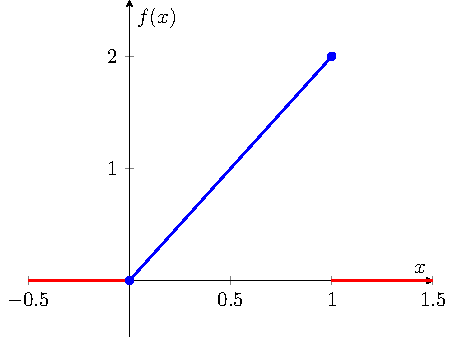
\includegraphics[width=0.5\textwidth]{Assets/Pdf/T9P2IA.pdf}
                \end{figure}

                b) Función de distribución:
                \[
                    F(x) = \int_{-\infty}^{x} 2u du
                    = 2 \int_{-\infty}^{x} u du =
                    \begin{cases}
                        0 & x < 0 \\
                        x^{2} & 0 \leq x \leq 1 \\
                        1 & x > 1                       
                    \end{cases}
                \]
                \begin{figure}[H]
                    \centering
                    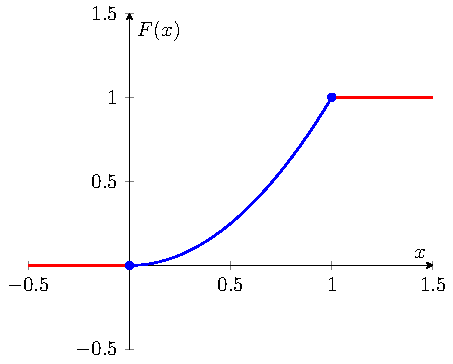
\includegraphics[width=0.5\textwidth]{Assets/Pdf/T9P2IB.pdf}
                \end{figure}
            }

        \newpage
        % - Problema 3
        \item Sea la función de distribución
        \[
            F(x) =
            \begin{cases}
                0 & x < 0 \\
                x & 0 \leq x \leq 1 \\
                1 & x > 1
            \end{cases}
        \]
        Determinar si se trata de la función de distribución de una variable aleatoria discreta o continua. Encontrar además la correspondiente función de probabilidad o densidad y graficarlas.
            % Respuestas:
            \vspace{\Aspace} \par
            { \color{azul} 
                Se trata de una variable continua. \par
                \vspace{\Aspace}
                a) Función de distribución:
                \begin{figure}[H]
                    \centering
                    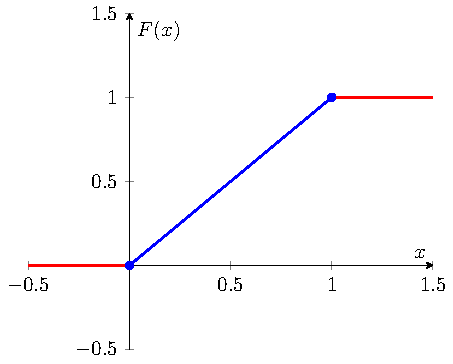
\includegraphics[width=0.5\textwidth]{Assets/Pdf/T9P3IA.pdf}
                \end{figure}

                b) Función de densidad:
                \[
                    \frac{d}{dx}F(x) = f(x) =
                    \begin{cases}
                        1   &   0 \leq x \leq 1     \\
                        0   &   \text{Otro caso}    \\
                    \end{cases}
                \]
                \begin{figure}[H]
                    \centering
                    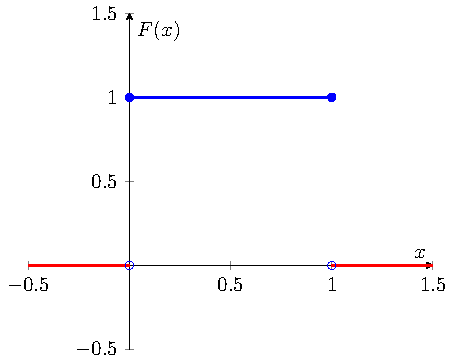
\includegraphics[width=0.5\textwidth]{Assets/Pdf/T9P3IB.pdf}
                \end{figure}
            }
    \end{enumerate}



    \newpage
    % ---------- Tarea 10 ----------
    \vspace{0.3cm}

    \begin{center}
        { \LARGE Tarea 10}
    \end{center}

    \begin{enumerate}
        % - Problema 1
        \item Encontrar el valor esperado y la desviación estándar de la función de densidad \par
        \[
            f(x) =
            \begin{cases}
                e^{-x} & x > 0 \\
                0 & \text{Otro caso}
            \end{cases}
        \]
            % Respuestas:
            \vspace{\Aspace}
            { \color{azul} 
                \begin{flushleft}
                    Valor esperado:
                \end{flushleft}
                \[
                    E[X] 
                    = \int_{0}^{\infty} xe^{-x}dx
                    = -xe^{-x} + \int_{0}^{\infty} e^{-x}dx
                    = -xe^{-x}-e^{-x} \Big|_{0}^{\infty}
                    = -\frac{x + 1}{e^{x}} \Big|_{0}^{\infty}
                    = 1
                \]

                \begin{flushleft}
                    Varianza:
                \end{flushleft}
                \[
                    \text{Var}[X]
                    = \int_{0}^{\infty} x^{2}e^{-x}dx - \int_{0}^{\infty}(x - 1)^{2}e^{-x}dx
                    = 2 - 1
                    = 1
                \]
            }

        % - Problema 2
        \vspace{\Pspace}
        \item Encontrar la función de densidad y distribución con $U \sim U(0, 4)$. Graficas ambas funciones y encontrar el valor esperado y la desviación estándar.
            % Respuestas:
            \vspace{\Aspace} \par
            { \color{azul} 
                Función de densidad:
                \[
                    f(x) = 
                    \begin{cases}
                        \frac{1}{4} &   0 < x < 4 \\
                        0           &   \text{Otro caso}
                    \end{cases}
                \]
                \begin{figure}[H]
                    \centering
                    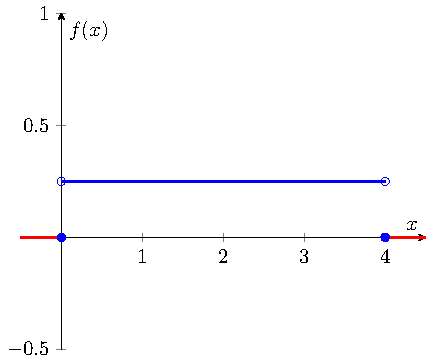
\includegraphics[width=0.5\textwidth]{Assets/Pdf/T10P2IA.pdf}
                \end{figure}
            }

        % - Problema 3
        \item Sea $X$ una variable aleatoria con distribución uniforme entre $-1$ y $1$. Demuestre lo siguiente
        \[
            E[X^{n}] =
            \begin{cases}
                0 & \text{si $n$ es impar}  \\
                \frac{1}{n + 1} & \text{si $n$ es par} \\
            \end{cases}
        \]
            % Respuesta:
            \vspace{\Aspace} \par
            { \color{azul} }

        % - Problema 4
        \item Usted no conoce el tiempo de respuesta a una solicitud, pero sabe que el mínimo posible es de 5 minutos y el máximo es de 25 minutos. ¿Qué distribución recomendaría utilizar? ¿Cuál es la probabilidad de recibir una respuesta entre 5 y 7 minutos? ¿Cuánto tiempo debe esperar en promedio?
    \end{enumerate}
\end{document}
